\section{Introduction}

\hl{should this stuff be moved up to 3LA?}

Machine learning (ML) and other
  high-performance computing (HPC)
  applications increasingly rely on
  specialized hardware accelerators to
  provide speed and energy efficiency~\cite{jouppi2017tpu, krizhevsky2012conv, reuther2019survey}.
This trend has highlighted the need
  for flexible accelerator support
  in domain-specific compilers like
  Halide~\cite{halide},
  TVM~\cite{chen2018tvm},
  TensorFlow/MLIR~\cite{tensorflow, mlir}, and
  PyTorch~\cite{pytorch}.

Adding accelerator support to
  an existing compiler typically
  uses custom pattern matching to
  map expensive tensor operations
  from applications down to
  accelerator invocations~\cite{
    yang2020interstellar, byoc}.
Pattern matching often additionally relies on
  various other transformations
  to canonicalize intermediate representations (IRs)
  %~\cite{??}
  and massage data layouts into
  formats matching accelerator requirements~\cite{nvidia2020nhwc}.
Even with these changes,
  users may need to manually modify their application to
  help the compiler discover opportunities
  for dispatching operations to accelerators, 
  such as by changing data types or unrolling loops.
    
In principle, term rewriting techniques~\cite{baader1998term}
  should be able to facilitate many of
  these transformation and mapping tasks
  within a compiler.
Halide and TVM already rely
  on extensive rewrite systems for
  optimizing scalar computations and
  simplifying loop bounds in order to
  support further downstream optimizations~\cite{newcomb2020halide-rewrite,
  hagedorn2020func-high-perf}.

Unfortunately, existing IRs in compilers for
  array/tensor programming DSLs tend to
  present abstraction and granularity mismatches
  that hamper term rewriting approaches.
Term rewriting is most easily applied in
  \textit{pure} (side effect--free) IRs
  that support equational reasoning.
At the same time,
  mapping to accelerators requires considering
  low-level hardware details like data layout.
Existing pure IRs for ML frameworks are used
  primarily for high-level transformations
  (e.g., type elaboration and inlining)
  and do not expose low-level data layout details~\cite{relay}.
On the other hand,
  IRs used for crucial lower-level optimizations like
  operator fusion must support
  precise reasoning about memory use,
  and therefore are typically impure,
  hampering term rewriting.% approaches.

To help mitigate such impedance mismatches,
  we present \textit{\g},\footnote{Publicly available at \url{https://github.com/gussmith23/glenside}.}
  a pure tensor program IR
  that enables hardware-level term rewriting.
\g is based on a simple
  \textit{access pattern} abstraction that
  supports expressing and reasoning about
  data layout transformations via
  syntactic rewrite rules.
% We moved this figure elsewhere in the thesis
%   \begin{wrapfigure}{r}{.5\textwidth}
%     \centering
%     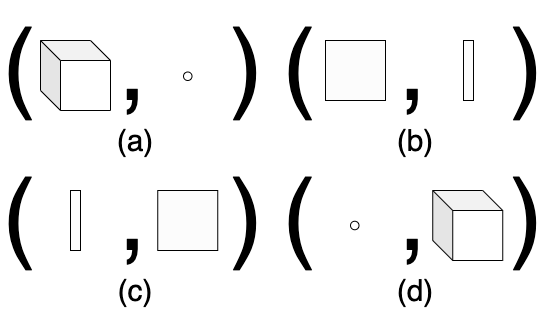
\includegraphics[width=.9\linewidth]{glenside/access-pattern-examples-2x2.png}
%     \caption{
%       Four access patterns,
%         representing different ways
%         a
%         tensor program
%         (or \textit{kernel})
%         might access
%         the same 3D tensor. 
%       For example, (c) represents
%         accessing a 3D tensor as
%         a vector of 2D matrices.}
%     \label{fig:access-pattern-examples}
%     \vspace{-1em}
% \end{wrapfigure}
When combined with standard arithmetic rewrites
  for per-tensor-element computations,
  access patterns enable implementing complex
  transformations for accelerator support as
  compositions of simple rewrites.

Tensors are traditionally characterized
  by their \textit{shape},
  an $n$-tuple 
  %in $\mathbb{N}^n$
  of positive integers
  indicating the size of each
  of a tensor's dimensions.
  % , e.g., $(x, y, z)$ for a 3D tensor.
Access patterns instead characterize
  each tensor with two shapes, e.g.,
  \accesspatternshape{x}{y, z}, separating
  the dimensions which are \textit{iterated over} from
  the dimensions which are \textit{computed on.}
Figure~\ref{fig:access-pattern-examples}(c)
  depicts an example where a 3D tensor's
  first dimension is iterated over and
  some computation applied to each
  corresponding 2D matrix.

We demonstrate how \g
  enables implementing representative
  hardware-level transformation via term rewriting,
  including mapping computations
  to systolic arrays~\cite{jouppi2017tpu}
  (a common hardware module in ML accelerators)
  and automatically discovering the
  \tcd{im2col} data layout transformation~\cite{im2col},
  which enables mapping 2D convolutions
  to matrix multiplication hardware.
In particular,
  by employing \textit{equality saturation}~\cite{willsey2021egg},
  these transformations ``fall out for free''
  (i.e., without any carefully crafted
  rewrite orderings~\cite{phase-ordering}),
  from a handful of general rewrites concerning tensor
  transposition, Cartesian product, dot product, etc.,
  expressed in terms of access patterns.

To summarize, the contributions of this chapter include:
\begin{itemize}
\item \textit{Access patterns},
  a tensor representation that employs a
  simple, extended tensor shape type to
  distinguish iteration and computation dimensions

\item The \g IR,
  a pure compiler IR that facilitates 
  term rewriting to enable support for
  specialized accelerators
  
\item A library of generic rewrites over \g programs
  
% \item Case studies demonstrating how
%   \g enables automatically discovering
%   key transformations for mapping
%   applications to custom accelerators
%   via equality saturation with the
%   \tcd{egg}~\cite{willsey2021egg} library.
\end{itemize}

\hl{i moved related work, so probably need to rework this}
The rest of this chapter is organized as follows:
Section~\hl{todo} provides background
  and briefly surveys closely related work.
Section~\hl{todo} motivates
  \g via a running example exploring
  pure matrix multiplication.
Section~\hl{todo} details the
  design and implementation of \g.
